\documentclass[oneside]{scrbook}

% Font-/Inputencoding.
\usepackage[T1]{fontenc}
\usepackage[utf8]{inputenc}

% Information for PDF file.
\usepackage{hyperref}
\hypersetup{
  pdfauthor={Paul Jungeblut},
  pdftitle={Text Indexing, Script/Summary},
  pdfsubject={Text Indexing, Script/Summary},
  pdfkeywords={Text Indexing, Lecture Notes, Script, Summary}
}

% Colors.
\usepackage{color}

% Separations in enumerations.
\usepackage{enumitem}
\setlist{itemsep=1pt,topsep=3pt}

% Use french spacing, even though its wrong for english sentences.
\frenchspacing

% Math.
\usepackage{amsmath}
\usepackage{mathtools}
\usepackage[standard,thmmarks]{ntheorem}
\usepackage{amssymb}
\theoremstyle{break}
\theorembodyfont{\normalfont}
\renewtheorem{Definition}{Definition}[chapter]
\renewtheorem{Example}[Definition]{Example}
\theorembodyfont{\itshape}
\renewtheorem{Theorem}[Definition]{Theorem}
\renewtheorem{Lemma}[Definition]{Lemma}

% Pseudocode.
\usepackage{algorithm}
\usepackage[noend]{algorithmic}
\algsetup{indent=2em}

% Nice table lines and page wide tables.
\usepackage{tabularx}
\usepackage{booktabs}

% Disable indentation of new paragraphs.
\usepackage{parskip}

% TikZ.
\usepackage{float}
\usepackage{tikz}
\usetikzlibrary{shapes.multipart}
\usetikzlibrary{calc}

% Bibliography.
\usepackage[style=numeric, backend=biber]{biblatex}
\addbibresource{references.bib}

% Index.
\usepackage{makeidx}
\makeindex

% Layout for introducing terms.
% Parameter 1: The term to print.
% Parameter 2: The term to put into the index.
\newcommand{\defi}[2]{\emph{\textcolor{blue}{#1}}\index{#2}}

% Oneliner to embed TikZ images.
% Parameter 1: Path to the image.
% Parameter 2: Caption.
% Parameter 3: The name of the label.
\newcommand{\drawing}[3]{
  \begin{figure}[htbp]
    \centering
    \input{#1}
    \caption{#2}
    \label{fig:#3}
  \end{figure}
}

\begin{document}
  \newpage
  \pagenumbering{arabic}
  % TODO (pjungeblut): Rename this chapter to something like "Basic
%                    Datastructures".
\chapter{Introduction}

\begin{Definition}
  Let $\Sigma = \{0, \ldots, \sigma - 1\}$ be a finite, ordered set. The elements of $\Sigma$ are called \defi{characters}{Character} or \defi{symbols}{Symbol} and $\Sigma$ is called an \defi{alphabet}{Alphabet} of size $\sigma$.
\end{Definition}

\begin{Definition}
  A \defi{string}{String} $S$ is a sequence of characters from an alphabet $\Sigma$.
  \begin{itemize}
    \item We usually use $n = \vert S \vert$ to be the length of the string.
    \item The $i$-th character of $S$ is $S[i]$. Indices are $0$-based.
    \item The substring from the $i$-th to the $j$-th character is $S[i..j]$.
    \item A substring with $i = 0$ is called \defi{prefix}{Prefix}. A substring with $j = n - 1$ is called \defi{suffix}{Suffix}.
    \item The $i$-th suffix is $S[i..n-1]$.
  \end{itemize}
\end{Definition}

\section{Suffix Tries}

\begin{Definition}
  Let $S = \{S_0, S_1, \ldots, S_{N-1}\}$ be a set of strings over an alphabet $\Sigma$. A \defi{trie}{Trie} $\mathcal{T}$ is a tree, where each node represents a different prefix in the set $S$. The root represents the empty prefix $\varepsilon$. Vertex $u$ representing prefix $Y$ is a child of vertex $v$ representing prefix $X$, if and only if $Y = Xc$ for some character $c \in \Sigma$. The edge $(v,u)$ is then labeled $c$.\\
  If $S$ is the set of all suffixes of a string $T$, the trie is called \defi{suffix trie}{Suffix Trie} of $T$.
\end{Definition}

\begin{Example}
  Figure~\ref{fig:suffixTrieExample} shows the suffix trie for the string "banana\$". The dollar sign "\$" is a sentinel that does not appear elsewhere in the text (and is lexicographically smaller than all other symbols). This guarantees, that no suffix is a prefix of another suffix and the suffix trie therefore has $n+1$ leaves.
  \drawing{basicDatastructures/tikz/suffixTrieExample.tex}{The suffix trie for the string "banana\$"}{suffixTrieExample}
\end{Example}

To construct a trie over string set $S = \{S_0, \ldots, S_{N-1}\}$, we need $\mathcal{O}(\vert S_0 \vert + \ldots + \vert S_{N-1} \vert)$ steps. This bound is tight: If all characters are pairwise distinct in all strings and no two strings share a character, than the number of different prefixes and therefore vertices is given by $1 + \sum_{i=0}^{N-1} \vert S_i \vert$, where the additional $1$ represents the empty prefix $\varepsilon$.\\
The time needed to search for a string $T$ of length $m = \vert T \vert$ in the trie depends on the implementation of the tree. If the children of each vertex are stored in a list, the time is in $\mathcal{O}(m\sigma)$. If the children are stored in a sorted array (using the order of the characters in the alphabet), the time is in $\mathcal{O}(m\log \sigma)$. By using a hash table and perfect hashing, the time is in $\mathcal{O}(m)$.

The space needed to store the suffix trie $\mathcal{T}$ for a string of length $n$ is in $\mathcal{O}{(n^2\log \sigma + n^2\log n)}$ bits. The first summand is the space needed to store the $\mathcal{O}(n^2)$ edge labels of one character $c \in \Sigma$ each. The second summand is the space needed to store the pointers to the children of each node.


\section{Suffix Trees}

\begin{Definition}
  A \defi{suffix tree}{Suffix Tree} $\mathcal{T}$ for a string $S$ is the suffix trie of $S$ where each unary path is converted into a single edge. Those edges are labeled with the concatenation of the characters from the replaced edges. The leaves of the suffix tree store the text position where the corresponding suffix starts.
\end{Definition}

\begin{Example}
  Figure~\ref{fig:suffixTreeExample} shows the suffix tree for the string "banana\$". It contains only $11$ vertices compared to the $23$ vertices of the suffix trie.
  \begin{figure}[htb]
    \centering
    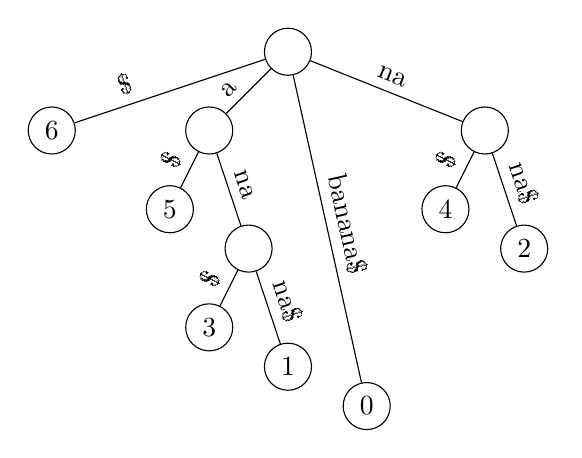
\begin{tikzpicture}
  \tikzstyle{vertex}=[circle,draw,minimum size=17pt,inner sep=0pt]
  \node[vertex] (epsilon) at (0,0) {};

  \node[vertex] (d) at (-3,-1) {6};
  \draw (epsilon) -- (d) node[above,sloped,pos=0.7] {\$};

  \node[vertex] (a) at (-1,-1) {};
  \draw (epsilon) -- (a) node[above,sloped,pos=0.7] {a};

  \node[vertex] (ad) at (-1.5,-2) {5};
  \draw (a) -- (ad) node[above,sloped,pos=0.5] {\$};

  \node[vertex] (ana) at (-0.5,-2.5) {};
  \draw (a) -- (ana) node[above,sloped,pos=0.5] {na};

  \node[vertex] (anad) at (-1,-3.5) {3};
  \draw (ana) -- (anad) node[above,sloped,pos=0.5] {\$};

  \node[vertex] (ananad) at (0,-4) {1};
  \draw (ana) -- (ananad) node[above,sloped,pos=0.5] {na\$};

  \node[vertex] (bananad) at (1,-4.5) {0};
  \draw (epsilon) -- (bananad) node[above,sloped,pos=0.5] {banana\$};

  \node[vertex] (na) at (2.5,-1) {};
  \draw (epsilon) -- (na) node[above,sloped,pos=0.5] {na};

  \node[vertex] (nad) at (2,-2) {4};
  \draw (na) -- (nad) node[above,sloped,pos=0.5] {\$};

  \node[vertex] (nanad) at (3,-2.5) {2};
  \draw (na) -- (nanad) node[above,sloped,pos=0.5] {na\$};
\end{tikzpicture}

    \caption{The suffix tree for the string "banana\$".}
    \label{fig:suffixTreeExample}
  \end{figure}
\end{Example}

The suffix array can be constructed in time $\mathcal{O}(n)$ with algorithms by \textsc{Weiner}\cite{Weiner1973}, \textsc{McCreight}\cite{McCreight1976} or \textsc{Ukkonen}\cite{Ukkonen1995}. It needs $\mathcal{O}(n\log n + n\log \sigma)$ bits. The first summand is the space needed for the pointers to the children and the indices stored in the leaves. The second summand is the space needed for the edge labels. To achieve this space, the edge labels must not be stored explicitly. Instead we can store pointers to the first and last position of the label in the text.

In practice, a suffix tree needs more than $20$ times the space of the original text. Based on the required functionality, this can even be worse.

\section{Bitvectors}

\begin{Definition}
  A \defi{bitvector}{Bitvector} $B$ is an array of bits that are compactly stored. A bitvector supports the following operations:
  \begin{itemize}
    \item $\mathrm{access}(i)$ returns the $i$-th element in $B$.
    \item $\mathrm{rank}(i)$ returns the number of set bits in the prefix $[0..i-1]$ of $B$.
    \item $\mathrm{select}(i)$ returns the position of the $i$-th set bit.
  \end{itemize}
\end{Definition}

\begin{Theorem}
  \label{thm:bitvectorRankConstantTime}
  The $\mathrm{rank}$-Operation on bitvectors can be done constant time and $o(n)$ additional space.\cite{Jacobson1989}
\end{Theorem}

\begin{Proof}
  Let $B$ be a bitvector of length $n$. Precompute the following information:
  \begin{enumerate}
    \item Divide $B$ into \emph{superblocks} $SB_1, \ldots, SB_{\lceil \frac{n}{L} \rceil}$ of size $L$.
    \item For each superblock $SB_j$ now store $\sum_{i=0}^{(j-1)L-1} B[i]$. This is the number of set bits in the first $j$ superblocks. For each superblock this needs $\mathcal{O}(\log n)$ bits of space.
    \item Now further divide each superblock $B_j$ into blocks $B_1^j, \ldots, B_{\lceil \frac{L}{S} \rceil}^j$ of size $S$.
    \item For each block $B_k^j$ of superblock $SB_j$ store $\sum_{i=(j-1)L}^{(j-1)L+kS-1} B[i]$. This is the number of set bits in the first $k$ blocks of superblock $SB_j$. For each block this needs $\mathcal{O}(\log L)$ bits.
  \end{enumerate}
  For a given $\mathrm{rank}(i)$ query we now calculate the corresponding superblock $SB_j$ and block $B_k$. We use the precomputed sums to get the number of set bits in all superblocks before $SB_j$ and all blocks before $B_k$. All thats missing now is the number of set bits in block $B_k$ until position $i$. If the blocks are small enough, this information can be precomputed efficiently for all possible blocks and positions (Four-Russians-Trick).

  We still need to choose $L$ and $S$:
  \begin{align}
    L &= \log^2 n \\
    S &= \frac{1}{2} \log n
  \end{align}
  The total amount of space needed is in $\mathcal{O}(\frac{n}{\log n} + \frac{n\log\log n}{\log n} + \sqrt{n}\log n\log\log n)$ bits.
\end{Proof}

\section{Wavelet Trees}

\begin{Definition}
  A \defi{wavelet tree}{Wavelet Tree} is a compact datastructure that stores a sequence $S$ generalizes the operations of a bitvector to an arbitrary alphabet.
  \begin{itemize}
    \item $\mathrm{access}(i)$ returns the $i$-th element of the sequence.
    \item $\mathrm{rank}_q(i)$ returns the number of occurrences of $q$ in the prefix $S[0..i-1]$.
    \item $\mathrm{select}_q(i)$ returns the position of the $i$-th occurrence of $q$ in $S$.
  \end{itemize}

  The root of the wavelet tree stores the whole sequence. Each vertex recursively divides its sequence to its two children. The left child contains the first half of the remaining alphabet, the right child contains the second half of the remaining alphabet. A bitvector in every vertex stores the corresponding child for each element.
\end{Definition}

\begin{Example}
  Figure~\ref{fig:waveletTreeExample} shows the wavelet tree for the string "abracadabra".
  \drawing{introduction/tikz/waveletTreeExample.tex}{The wavelet tree for the string "abracadabra".}{waveletTreeExample}
\end{Example}

\begin{Lemma}
  A wavelet tree can be stored in $n\lceil\log\sigma\rceil$ bits space.
\end{Lemma}

\begin{Proof}
  The wavelet tree has height $\lceil\log\sigma\rceil$ and stores $n$ bits on every layer (maybe even less on the last layer). Therefore $n\lceil\log\sigma\rceil$ bits are needed to store the bitvectors. A wavelet tree can be implemented fully via bitvectors and does not need any pointers.
\end{Proof}

% TODO (pjungeblut): Describe implementation via bitvectors.
% TODO (pjungeblut): Describe implementation of operations.


  \printindex
  \printbibliography
\end{document}
